\chapter{DESENVOLVIMENTO}
\label{cap:desenvolvimento}

Neste capítulo serão apresentados os projetos e tecnologias utilizadas durante o tempo de estágio experienciado.

Na sua grande maioria, os projetos do LEMAF são sistemas webs, contituidos de uma aplicação backend e uma frontend.

O backend durante o desenvolvimento muitas vezes é rodado no computador do proprio dev, porém quando há nescessidade de serem feitos testes, é criado um servidor dentro da rede local para que possam ser efetuados os mesmo, sendo mais precisos por conta de estarem em um servidor.

A infraestrutura de servidores do LEMAF muitas vezes são servidores com diversas maquinas, todas rodando ngnix para prover as aplicações.

O frontend geralmente seguia o mesmo processo do backend, porém quando ia para alguma maquina externa, era criado alguma configuração para que o backend servisse o frontend, evitando assim problemas de CORS.

Já o banco de dados era controlado por um DBA(Database Administrator), que criava e gerenciava toda a estrutura de banco, sendo somente nescessario aos desenvolvedores, discutir melhores soluções e criar tarefas para os mesmos.

Durante o ano como estagiario, participei de todos squads, trabalhando com diversos times, projetos e tecnologias.

Em minha primeira equipe(Squad 1 - Carreta Furacão), tive como tecnologias nescessarias JAVA(backend) e Angular(Frontend), para que fosse possivel evoluir os projetos do Cadastro Ambiental Rural, incluindo os projetos SICAR, Central do Responsavel Tecnico, Central do Proprietario, PRA-OFF.

\begin{figure}[H]
\centering
\caption{SICAR-PA} %legenda
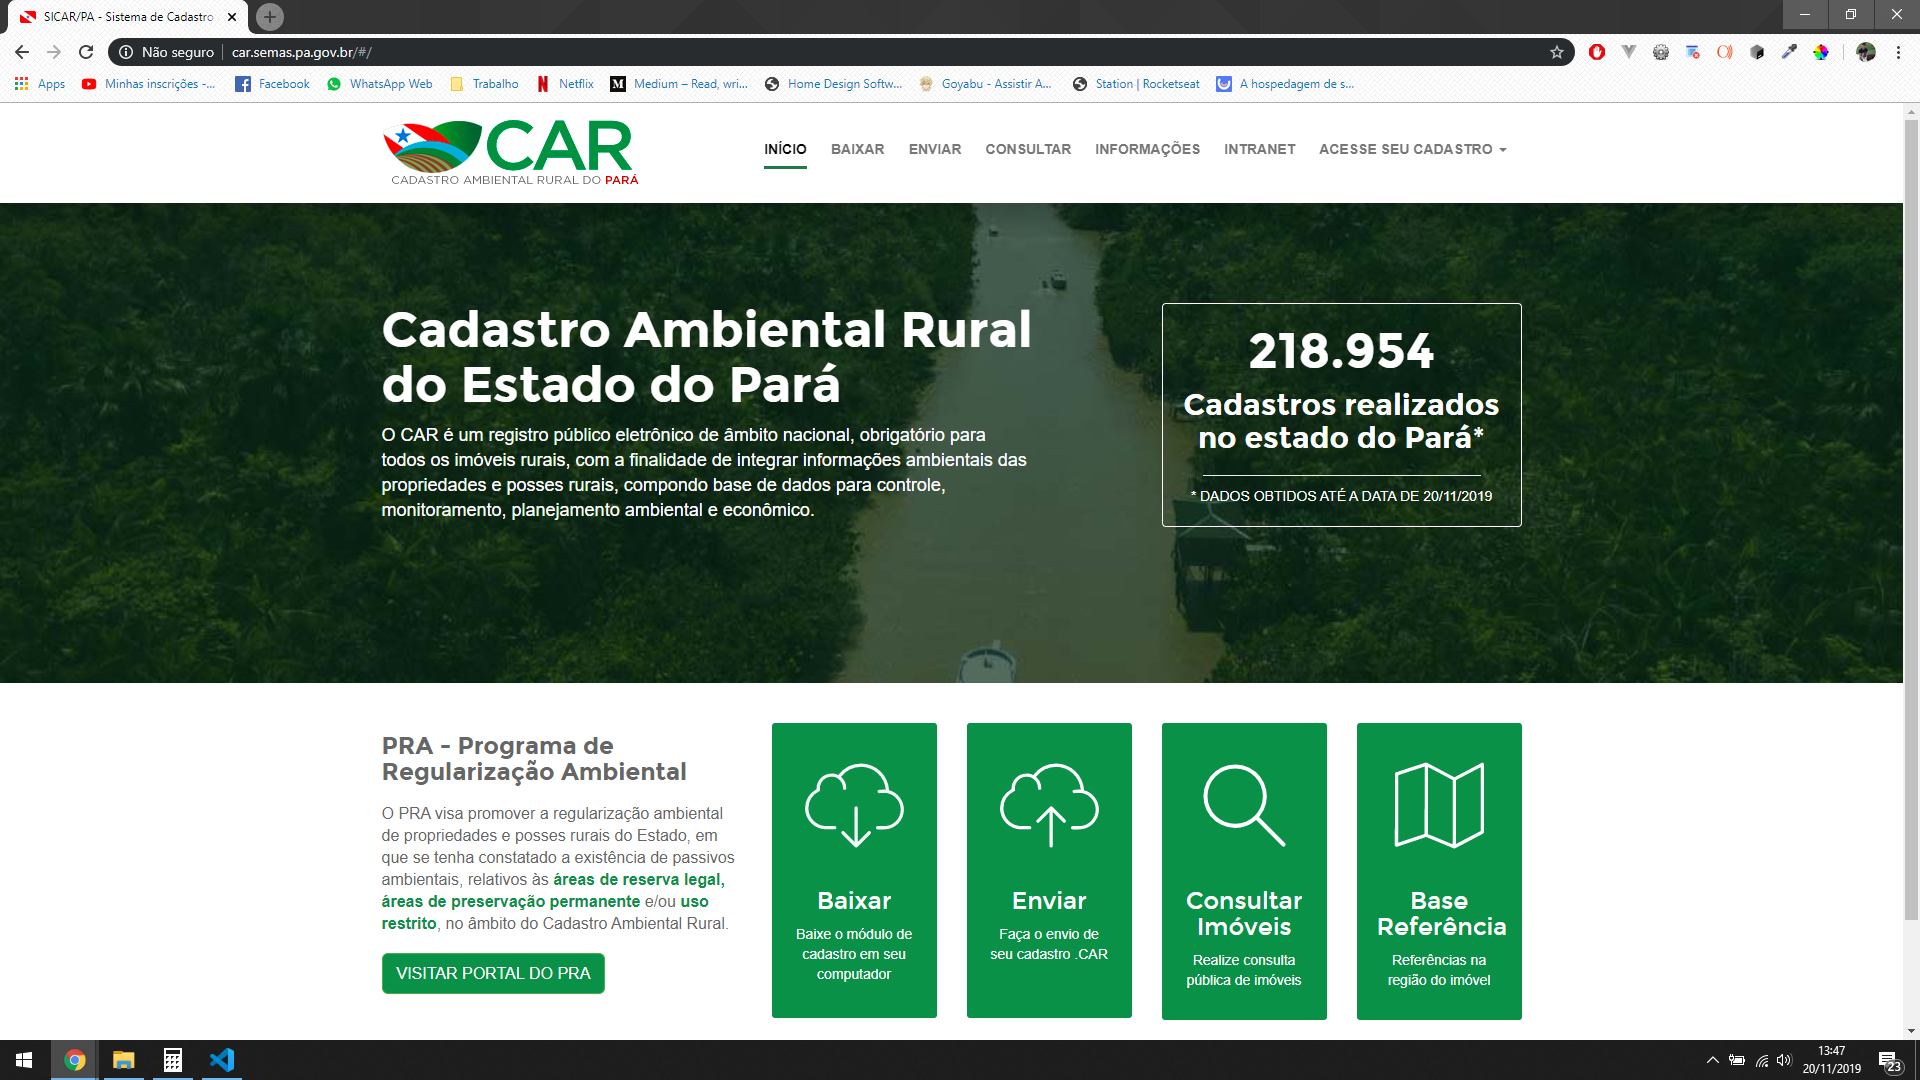
\includegraphics[scale=0.3]{SICAR}\\  % o 0.9 indica 90% do tamanho original
% pdfLaTeX aceita figuras no formato PNG, JPG ou PDF
% figuras vetoriais podem ser exportadas para eps e depois convertidas para pdf usando epstopdf
{\small Fonte: http://car.semas.pa.gov.br/#/} %Fonte da imagem
\label{fig:exemplo} %rotulo para refencia
\end{figure}

O projeto do SICAR tinha como objetivo informar e controlar os cadastros ambientais rurais feitos no estado do pará, sendo nescessaria algumas integraçoes com os modulos do SICAR federal e as Centrais ligadas ao PRA.

\begin{figure}[H]
\centering
\caption{PRA-OFF} %legenda
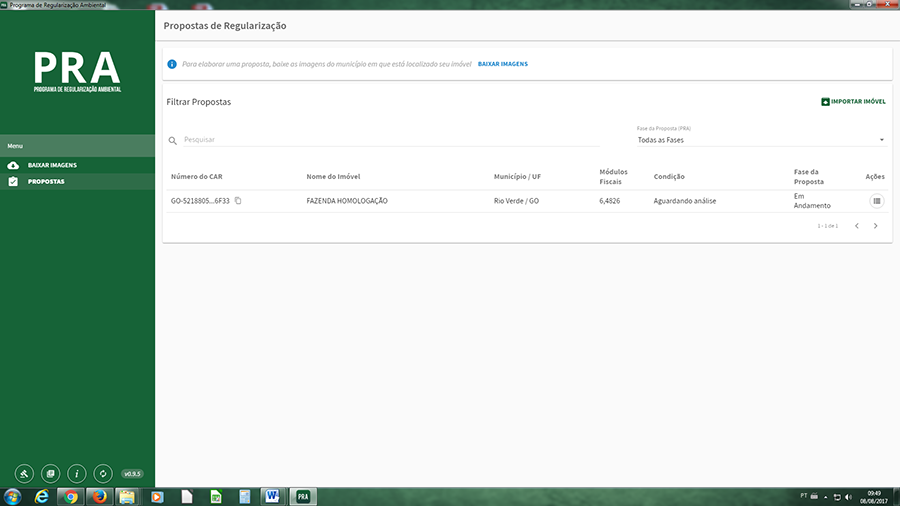
\includegraphics[scale=0.5]{pra-off}\\  % o 0.9 indica 90% do tamanho original
% pdfLaTeX aceita figuras no formato PNG, JPG ou PDF
% figuras vetoriais podem ser exportadas para eps e depois convertidas para pdf usando epstopdf
{\small Fonte: http://www.cprh.pe.gov.br/Controle_Ambiental/Sistema%20Nacional%20de%20Cadastro%20Ambiental%20Rural%20-%20SICAR/PRA/43052%3B53356%3B480802%3B0%3B0.asp} %Fonte da imagem
\label{fig:exemplo} %rotulo para refencia
\end{figure}

Já o projeto do PRA, não era possiveis tais integrações, pois ele era um modulo offline, sendo possivel a utilização sem internet. Para o desenvolvimento do mesmo, foi nescessario estudar sobre electron, uma ferramenta que possibilita criar modulos web em aplicações offiline.

Após 5 meses a equipe foi quebrada em duas e então foi feita uma redistribuição de projetos e acabei indo para a tribo Runners. Os projetos principais que contribui durante esse periodo foram o Consulta Publica - PARÁ e relatórios do PRA.

\begin{figure}[H]
\centering
\caption{Consulta publica} %legenda
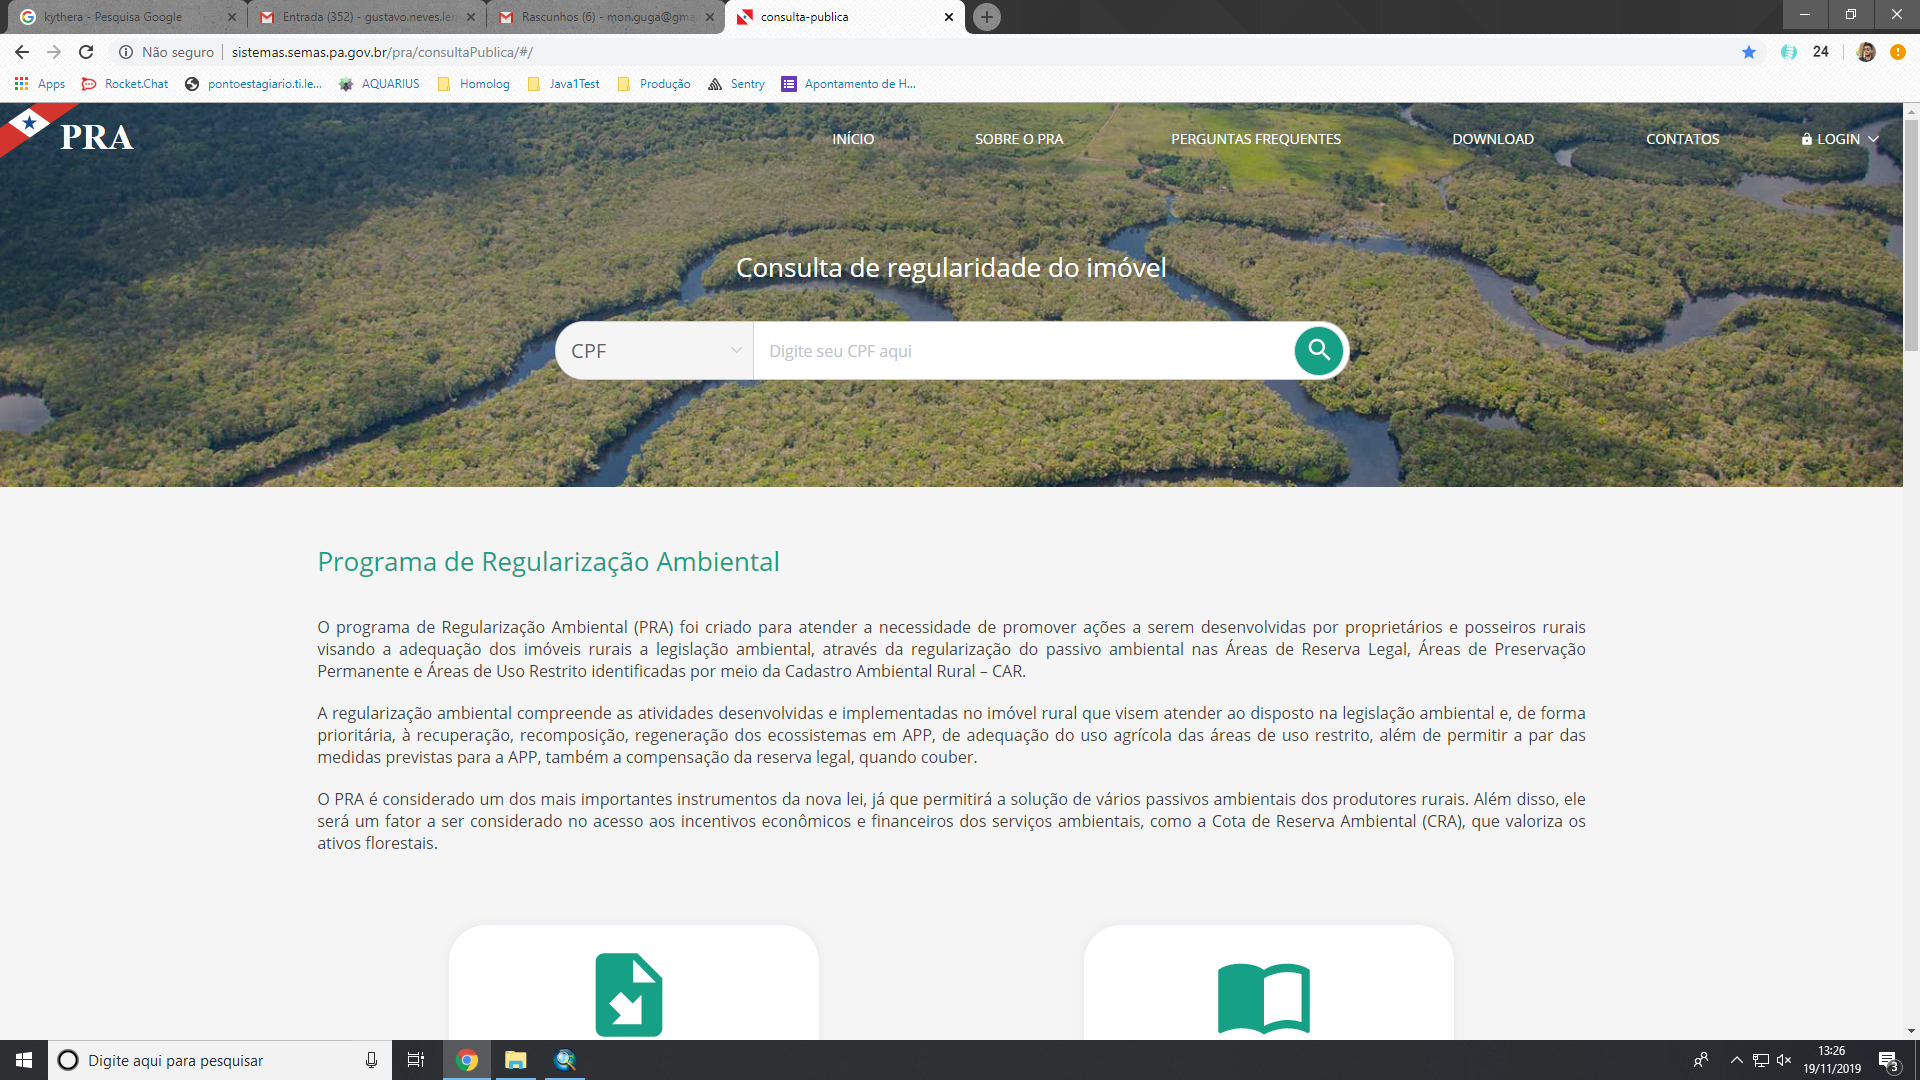
\includegraphics[scale=0.22]{consulta-publica}\\  % o 0.9 indica 90% do tamanho original
% pdfLaTeX aceita figuras no formato PNG, JPG ou PDF
% figuras vetoriais podem ser exportadas para eps e depois convertidas para pdf usando epstopdf
{\small Fonte: http://sistemas.semas.pa.gov.br/pra/consultaPublica/#/} %Fonte da imagem
\label{fig:exemplo} %rotulo para refencia
\end{figure}

O projeto consulta publica foi o primeiro projeto que tive como objetivo a refatoração, pois o projeto era antigo, utilizava uma das primeiras versões de VueJs no frontend e tinha o layout bem ruim.
Foi a primeira obrigação que tive total responsabilidade, tinha que migrar todo o sistema para VueJs 2.0 e refatorar o frontend.

Como era minha primeira experiencia com o framework VueJs, o projeto foi bem demorado, tive suporte do meu time que me tutoriava sobre arquitetura, padrões de projetos, boas praticas.
Para melhor aprendisado meu e um controle sobre codigos ruins, todas modificações feitas por mim sempre passavam por um Code Review e só quando aprovadas, eram enviadas para o projeto. 

O projeto consulta publica tinha como objetivo mostar para os proprietários de imoveis rurais suas areas desmatadas, se seus imoveis estavam de acordo com as regularizações ambientais e informações gerais sobre a geometria e hidrografia do terreno.


\begin{figure}[H]
\centering
\caption{Relatórios do PRA} %legenda
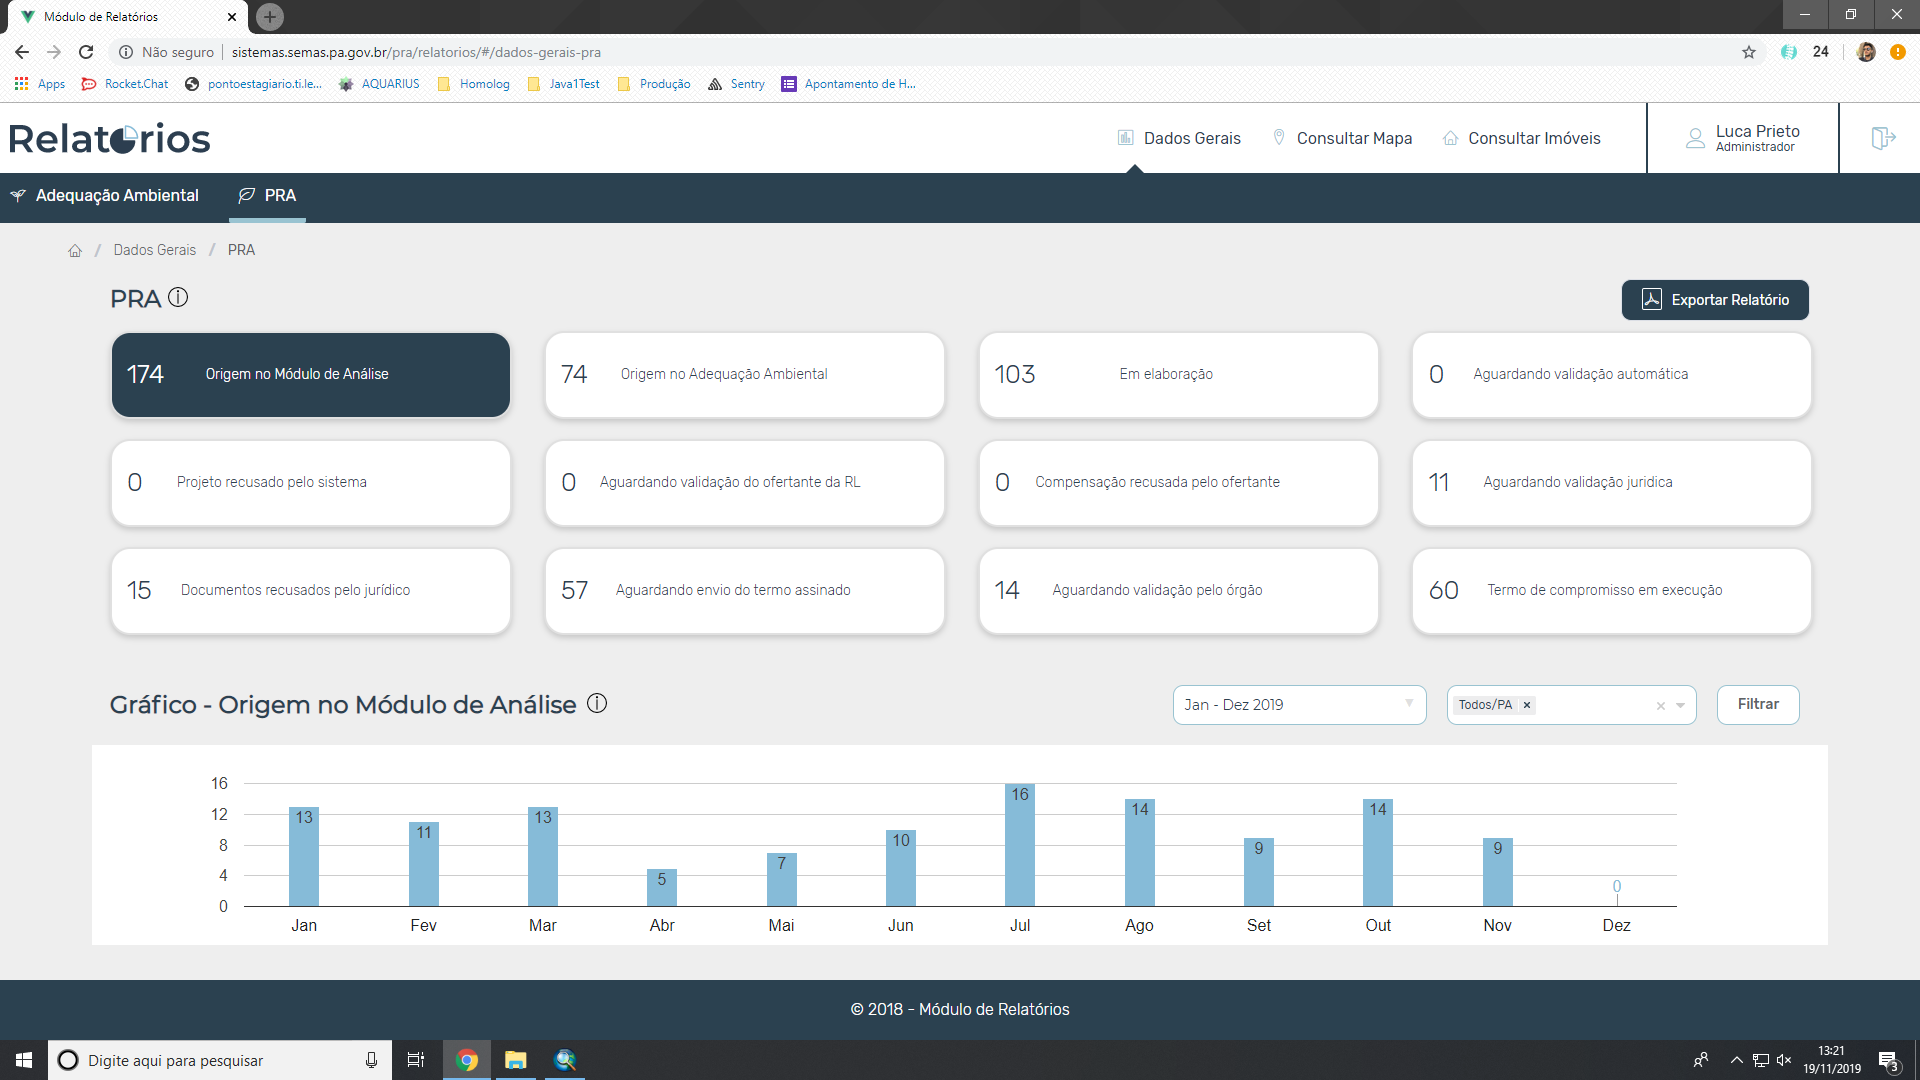
\includegraphics[scale=0.22]{relatorios-pra}\\  % o 0.9 indica 90% do tamanho original
% pdfLaTeX aceita figuras no formato PNG, JPG ou PDF
% figuras vetoriais podem ser exportadas para eps e depois convertidas para pdf usando epstopdf
{\small Fonte: http://sistemas.semas.pa.gov.br/pra/relatorios/#/dados-gerais-adequacao-ambiental} %Fonte da imagem
\label{fig:exemplo} %rotulo para refencia
\end{figure}

O projeto de relatorios foi o primeiro projeto que tive a honra de iniciar, com uma equipe formada de 4 pessoas (2 desenvolvedores, uma tester e uma PO).
O projeto consistia em uma plataforma de relatorios sobre o Programa de regularização ambiental e Adequação ambiental.

A escolha da tecnologia foi deixada como escolha nossa, então pela otima experiências com VueJs e o alto desempenho do framework , escolhemos o mesmo para o frontend.
porém pelo baixo conhecimento sobre backend, a escolha da tecnologia foi feita pelo outro Dev da equipe, que escolheu Spring Boot.
Como só tinha evoluido softwares e nunca começado um, houveram diversos gargalos no desenvovimento, como criação de ambientes, scripts para automatização de deploy entre outros.

porém Após 2 meses, fui transferido para uma equipe especial que não possuia tribo e que estava precisando de alguem com conhecimento em frontend e então me convocaram.
O projeto era uma POC(Prova de conceito) que uma empresa ligada a Agronomia havia comprado. Com prazos curtissimos e complexidade alta, o projeto foi um dos mais dificeis que já havia trabalhado.
O projeto foi todo construido utilizando componentização, com o backend feito com uma arquitetura bem definida e documentada para que fosse possivel evoluir sem dificuldade. Graças a esse começo bem estruturado o projeto ocorreu bem.

Após esse projeto, fui alocado na tribo Atlantica onde trabalhei juntamente com outro desenvolvedor em um projeto, o SEIRH-CMS.

\begin{figure}[H]
\centering
\caption{SEIRH-CMS} %legenda
\includegraphics[scale=0.22]{SEIRH-CMS}\\  % o 0.9 indica 90% do tamanho original
% pdfLaTeX aceita figuras no formato PNG, JPG ou PDF
% figuras vetoriais podem ser exportadas para eps e depois convertidas para pdf usando epstopdf
{\small Fonte: http://monitoramento.semas.pa.gov.br/SEIRHCMS} %Fonte da imagem
\label{fig:exemplo} %rotulo para refencia
\end{figure}

O projeto do SEIRH-CMS era um gerenciador de conteudo da aplicação SEIRH(Sistema Estadual de Informações Sobre Recursos Hídricos do Pará).
A plataforma web do SEIRH já existia, porém não havia comunicação com um backend, então seu conteudo não era gerenciavel, logo, havia a nescessidade de uma refatoração total do sistema.

\begin{figure}[H]
\centering
\caption{SEIRH} %legenda
\includegraphics[scale=0.22]{SEIRH}\\  % o 0.9 indica 90% do tamanho original
% pdfLaTeX aceita figuras no formato PNG, JPG ou PDF
% figuras vetoriais podem ser exportadas para eps e depois convertidas para pdf usando epstopdf
{\small Fonte: http://monitoramento.semas.pa.gov.br/SEIRH} %Fonte da imagem
\label{fig:exemplo} %rotulo para refencia
\end{figure}

O prazo não diminui e então foi adicionado essa tarefa de refatoração ao nosso time.
Como já havia mais conhecimento sobre backend e toda tribo Atlantica ser constituida de desenvolvedores DotNet, resolvemos utilizar o framework DotNet Core 2.0, que 
provia diversas funcionalidades e atendia as nossas expectativas e nescessidades.
Já o frontend continuou sendo feito com VueJs, uma vez que acabavamos de sair de projetos feitos com VueJs.

O projeto tinha como prazo 2 sprints(1 mes), um tempo muito curto e como era nescessaria a entrega, optamos por utilizar um quadro kambam.
Foi minha primeira experiencia tomando liderança em prioridades das atividades, definição das atividades e organização no geral.

O projeto foi finalizado com exelencia no prazo estipulado e graças a isso, fui realocado em um time que já trabalhava com DotNet e precisava de mais um desenvolvedor.

O projeto desta vez fazia parte de um grande complexo de plataformas que havia sido encomendado por uma empresa de agronomia e tinha muitos componentes de frontend parecidos.

Dai surgiu a iniciativa por parte minha e de outro desenvolvedor, de iniciar a construção do Design System da empresa.
Dai surgiu o Cria Design System, que é uma biblioteca de componentes UI para ReactJs.

Todos componentes eram criados pelo design do projeto, definido comportamentos e animações e depois desenvolvido. Para a visualização dos componentes separadamente, utilizamos o StoryBook,
que cria e organiza o catalogo de componentes e então para que essa biblioteca fosse compartilhada por toda empresa e não surgissem varios bugs, foram implementados testes automatizados para todos componentes e com uma nessesidade de cobertura de no minimo 80\%.

\begin{figure}[H]
\centering
\caption{Cria Design System} %legenda
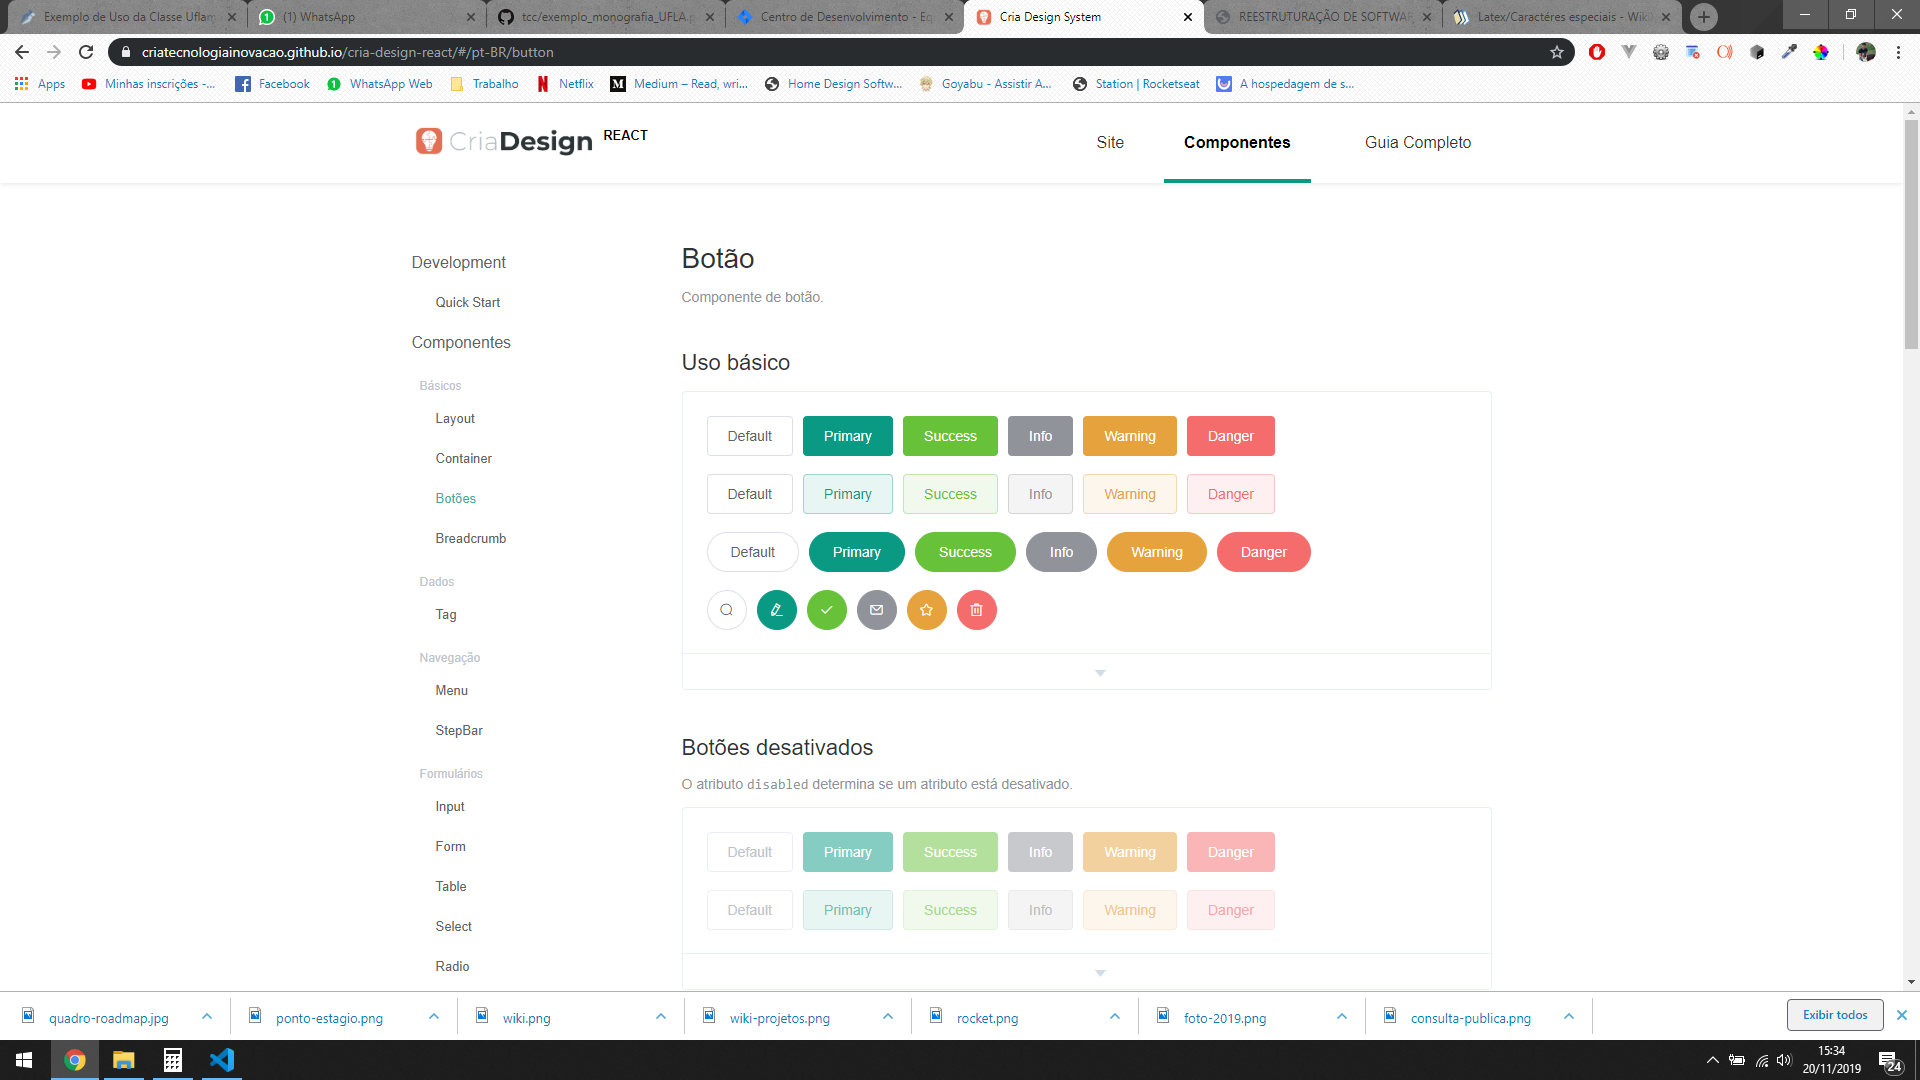
\includegraphics[scale=0.3]{cria-design}\\  % o 0.9 indica 90% do tamanho original
% pdfLaTeX aceita figuras no formato PNG, JPG ou PDF
% figuras vetoriais podem ser exportadas para eps e depois convertidas para pdf usando epstopdf
{\small Fonte: https://criatecnologiainovacao.github.io/cria-design-react/#/pt-BR/button} %Fonte da imagem
\label{fig:exemplo} %rotulo para refencia
\end{figure}

Após ajudar com o começo do projeto e facilitar o desenvolvimento do mesmo, fui incorporado a uma equipe na mesma tribo e cuidava de alguns projetos como o SIOUT e SIGER-PA.

\begin{figure}[H]
\centering
\caption{sigerpa} %legenda
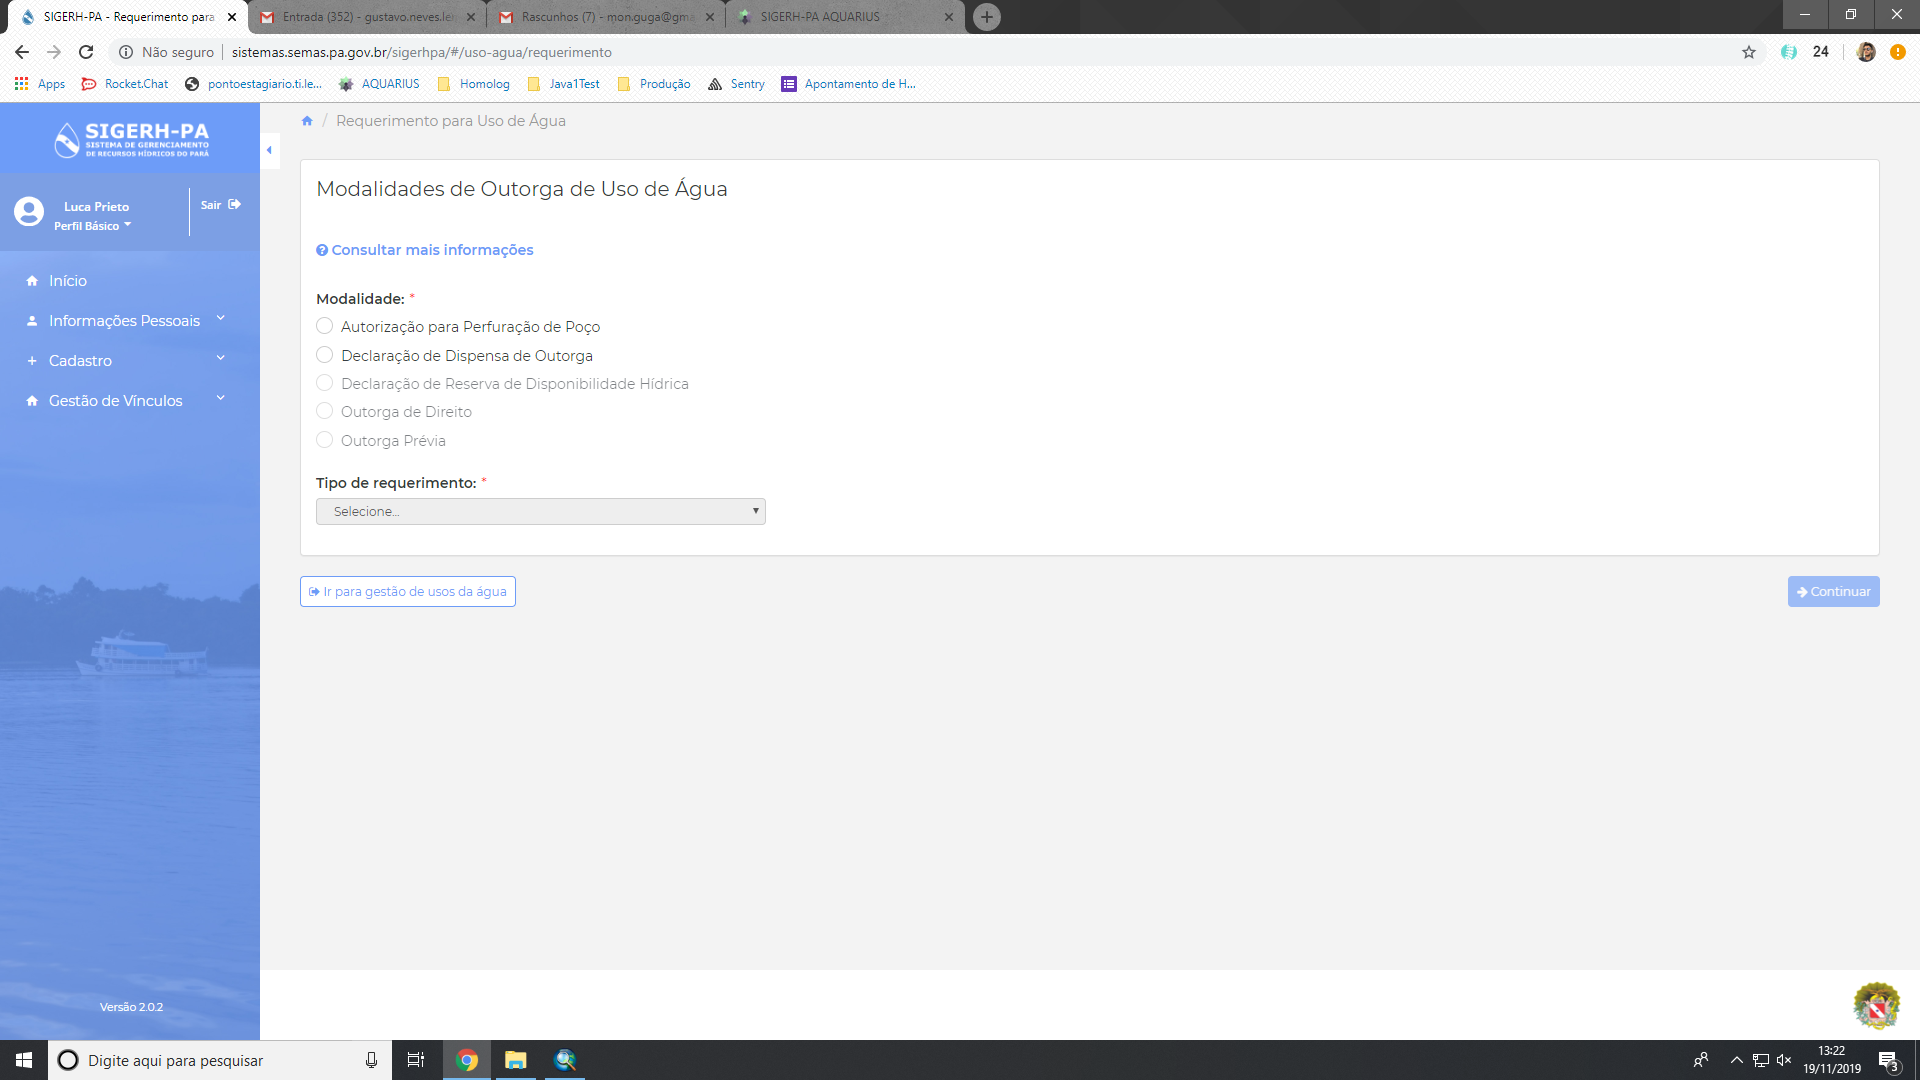
\includegraphics[scale=0.222]{sigerpa}\\  % o 0.9 indica 90% do tamanho original
% pdfLaTeX aceita figuras no formato PNG, JPG ou PDF
% figuras vetoriais podem ser exportadas para eps e depois convertidas para pdf usando epstopdf
{\small Fonte: http://sistemas.semas.pa.gov.br/sigerhpa/} %Fonte da imagem
\label{fig:exemplo} %rotulo para refencia
\end{figure}

O projeto do SIGER-PA(Sistema de Gerenciamento de Recursos Hídricos do Pará) é uma plataforma de cadastro e regularização de recursos hidricos(poços artesianos, nascentes e outros).
O projeto usava como backend o framework DotNet Framework 4.0 e como frontend AngularJs.

Até o fim do meu estágio, tive como tarefa evoluir e corrigir este sistema, que possuia varios problemas e alta complexidade por ser um sistema muito grande.
